\documentclass[]{thesis-ekf}
\usepackage[T1]{fontenc}
\PassOptionsToPackage{defaults=hu-min}{magyar.ldf}
\usepackage[magyar]{babel}
\usepackage{mathtools,amssymb,amsthm,pdfpages}
\footnotestyle{rule=fourth}

\newtheorem{tetel}{Tétel}[chapter]
\theoremstyle{definition}
\newtheorem{definicio}[tetel]{Definíció}
\theoremstyle{remark}
\newtheorem{megjegyzes}[tetel]{Megjegyzés}

\begin{document}

\institute{Matematikai és Informatikai Intézet}
\title{PokerParty}
\author{Szabó Márk\\programtervező informatikus Bsc.}
\supervisor{Troll Ede\\tanársegéd}
\city{Eger}
\date{2025}
\maketitle

\tableofcontents

\chapter*{Bevezetés}
\addcontentsline{toc}{chapter}{Bevezetés}

\chapter{Technológiai áttekintés}

\section{Enginek}
Általános leírás és összehasonlítás az API alapú fejlesztéssel

\subsection{Unreal}
\subsection{Godot}
\subsection{Unity}

\section{Többjátékos technológia a játékfejlesztésben}

\subsection{Korai megoldások}
Helyi többjátékos mód
\subsection{Kliens-Szerver}
\subsection{Dedikált szerver}
\subsection{Peer-to-Peer (P2P)}

\chapter{Rendszerterv}
Azok az elemek, amiket tanultatok RFT-n, azok kerülnek ide

\section{Rendszer célja}
\section{Követelmények}
\section{Architekturális terv}
PC unity, Mobile unity, SharedDLL
\section{Használt fejlesztői eszközök}

\chapter{Saját szoftver megvalósítása}

\section{Többjátékos kapcsolat megvalósítása}

\subsection{Kapcsolat kezelése a PC oldalon}
\subsection{Kapcsolat kezelése a Mobile oldalon}

\section{Texas Hold'Em}

\subsection{Szabályok ismertetése}
\subsection{Használt kézkiértékelő algoritmus}

\section{Játékmenet megvalósítása}

\subsection{Modul1}
\subsection{Modul2}

\chapter{Tesztelés}

\section{SharedDLL tesztelése}
\section{PC játék tesztelése}
\section{Mobile játék tesztelése}
\section{Általános tesztelés}

\chapter*{Összegzés}
\addcontentsline{toc}{chapter}{Összegzés}

\begin{thebibliography}{2}
\addcontentsline{toc}{chapter}{\bibname}

\end{thebibliography}

% Aláírt, szkennelt nyilatkozat beillesztése a szakdolgozat végére
%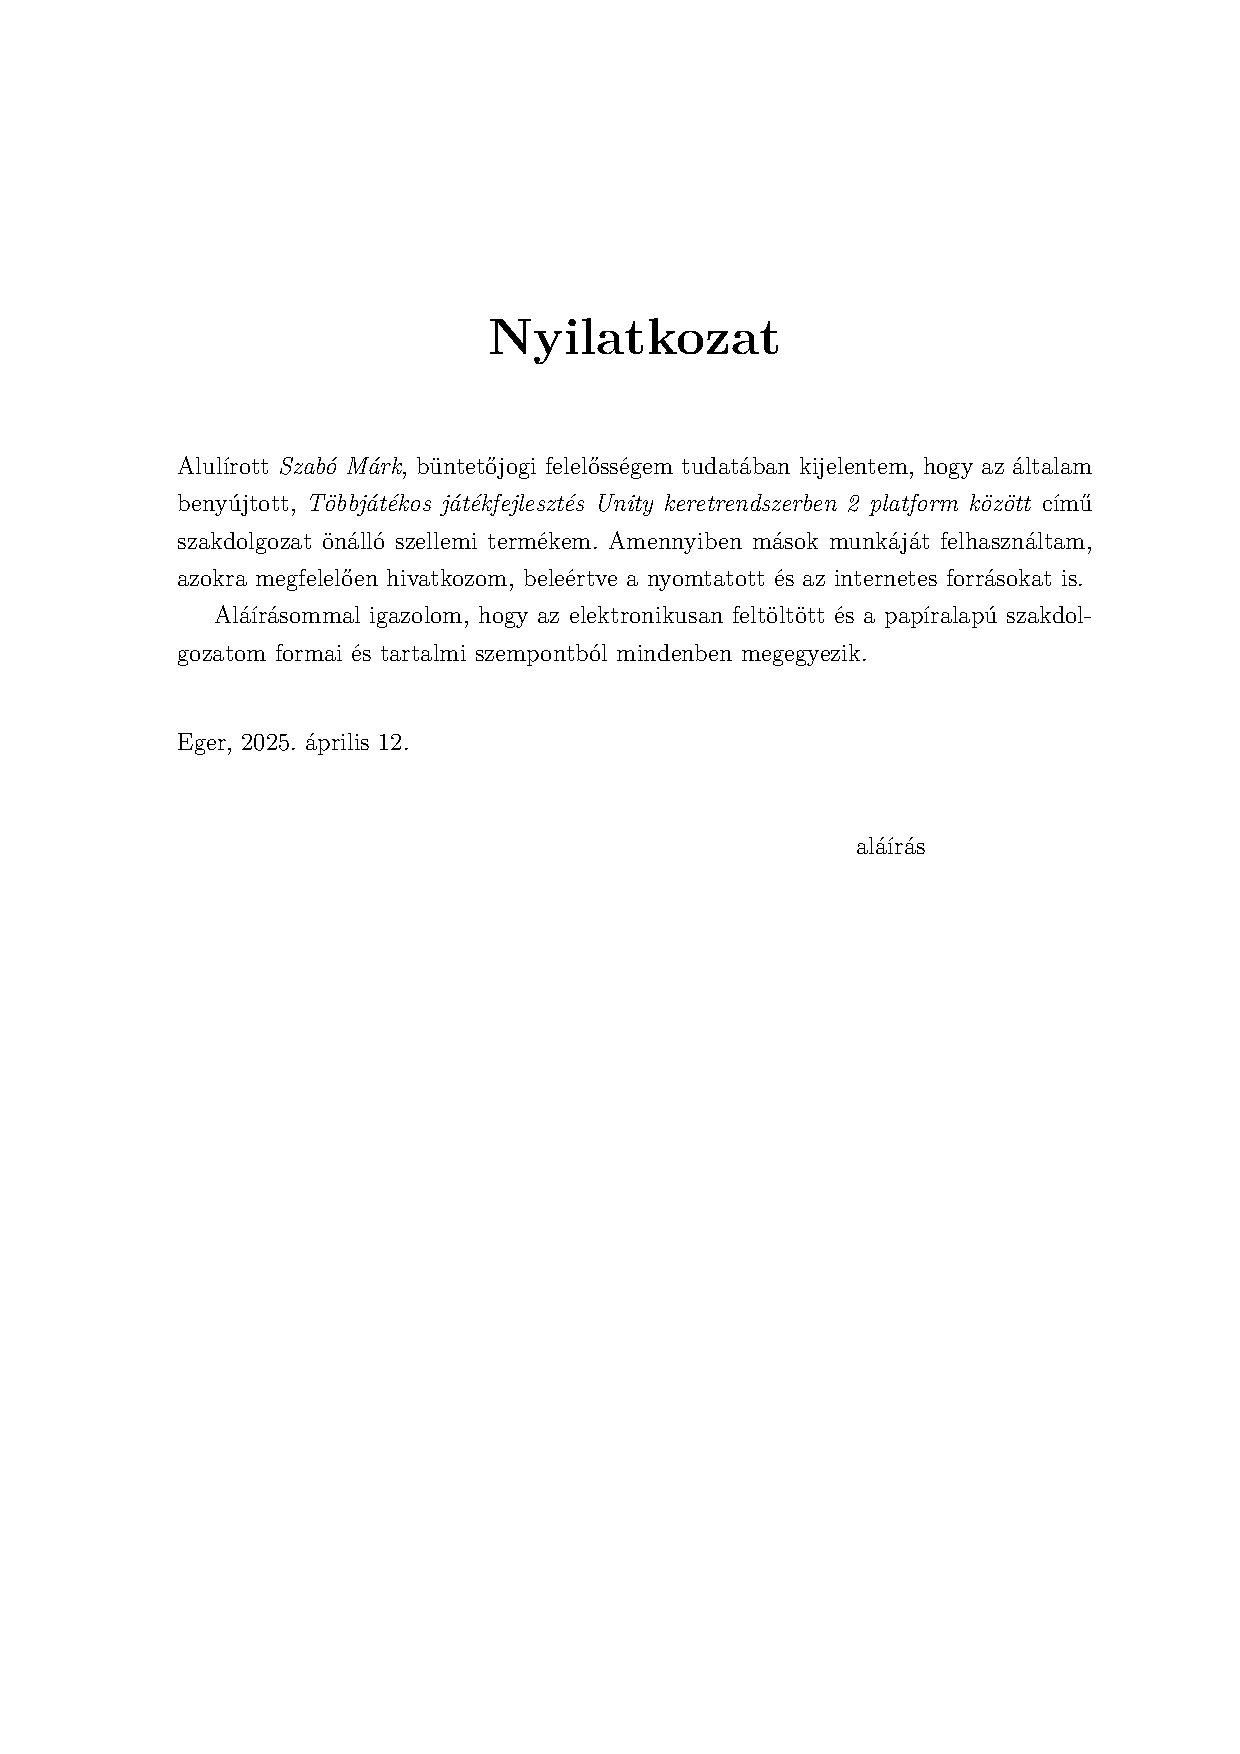
\includepdf{nyilatkozat/nyilatkozat.pdf}
\end{document}